% =====================================================================
% AI-POWERED SMART GLASSES USING ESP32-CAM
% VTU Mini Project Report - LaTeX Source
% Department of Computer Science and Engineering
% (IoT, CyberSecurity including Blockchain)
% Alva's Institute of Engineering & Technology, Moodbidri
% Academic Year: 2025-2026
% =====================================================================

\documentclass[12pt,a4paper]{report}
\usepackage[left=1.25in,right=1in,top=1in,bottom=1in]{geometry}
\usepackage{times}
\usepackage{graphicx}
\usepackage{fancyhdr}
\usepackage{titlesec}
\usepackage{setspace}
\usepackage{hyperref}
\usepackage{enumitem}
\usepackage{array}
\usepackage{longtable}
\usepackage{xcolor}
\usepackage{tikz}
\usepackage{background}
\usepackage{ulem}
\usepackage{tabularx}
\usepackage{multirow}
\usepackage{caption}

\onehalfspacing

% ===================== COLOR DEFINITIONS =====================
\definecolor{darkred}{RGB}{139,0,0}
\definecolor{darkblue}{RGB}{0,0,139}
\definecolor{darkgreen}{RGB}{0,128,0}

% ===================== PAGE BORDER (Front Matter Only) =====================
% Double-line black border for front matter pages
\newcommand{\enableborder}{%
\backgroundsetup{
  scale=1,
  color=black,
  opacity=1,
  angle=0,
  position=current page.center,
  vshift=0cm,
  hshift=0cm,
  contents={%
    
\begin{tikzpicture}[remember picture, overlay]
      \draw[black, line width=2pt] 
        ([shift={(0.5cm,-0.5cm)}]current page.north west) 
        rectangle 
        ([shift={(-0.5cm,0.5cm)}]current page.south east);
      \draw[black, line width=0.5pt] 
        ([shift={(0.65cm,-0.65cm)}]current page.north west) 
        rectangle 
        ([shift={(-0.65cm,0.65cm)}]current page.south east);
    \end{tikzpicture}%
  }
}}
\newcommand{\disableborder}{%
\backgroundsetup{contents={}}%
}

% ===================== PAGE STYLES =====================
% Default: no header/footer for front matter
\pagestyle{empty}

% Chapter pages: dark red header and footer with rules
\fancypagestyle{chapterpages}{
  \fancyhf{}
  \fancyhead[L]{\small\color{darkred}\textbf{AI-POWERED SMART GLASSES USING ESP32-CAM}}
  \fancyfoot[L]{\footnotesize\color{darkred}\textbf{Dept. of CS\&E (IoT, CyberSecurity including Blockchain)}}
  \fancyfoot[R]{\small\textbf{| \thepage}}
  \renewcommand{\headrulewidth}{1.5pt}
  \renewcommand{\footrulewidth}{1.5pt}
  \renewcommand{\headrule}{{\color{darkred}\hrule height 1.5pt}}
  \renewcommand{\footrule}{{\color{darkred}\vspace{2pt}\hrule height 1.5pt\vspace{4pt}}}
}

% Override 'plain' style used on chapter-opening pages
\fancypagestyle{plain}{
  \fancyhf{}
  \fancyhead[L]{\small\color{darkred}\textbf{AI-POWERED SMART GLASSES USING ESP32-CAM}}
  \fancyfoot[L]{\footnotesize\color{darkred}\textbf{Dept. of CS\&E (IoT, CyberSecurity including Blockchain)}}
  \fancyfoot[R]{\small\textbf{| \thepage}}
  \renewcommand{\headrulewidth}{1.5pt}
  \renewcommand{\footrulewidth}{1.5pt}
  \renewcommand{\headrule}{{\color{darkred}\hrule height 1.5pt}}
  \renewcommand{\footrule}{{\color{darkred}\vspace{2pt}\hrule height 1.5pt\vspace{4pt}}}
}



% ===================== CHAPTER FORMATTING =====================
\titleformat{\chapter}[display]
{\normalfont\Large\bfseries}{CHAPTER \thechapter}{12pt}{\Large\MakeUppercase}
\titlespacing*{\chapter}{0pt}{-20pt}{20pt}

% ===================== HYPERREF SETUP =====================
\hypersetup{
  colorlinks=false,
  pdfborder={0 0 0}
}

\begin{document}

% ================================================================
%                    FRONT MATTER (with border)
% ================================================================
\enableborder

% =================== TITLE PAGE ===================
\thispagestyle{empty}
\begin{center}
\vspace*{0.1cm}
{\color{darkblue}\textbf{\large VISVESVARAYA TECHNOLOGICAL UNIVERSITY,}}\\
{\color{darkblue}\textbf{\large BELAGAVI -- 590018}}\\[0.2cm]

% === VTU LOGO ===
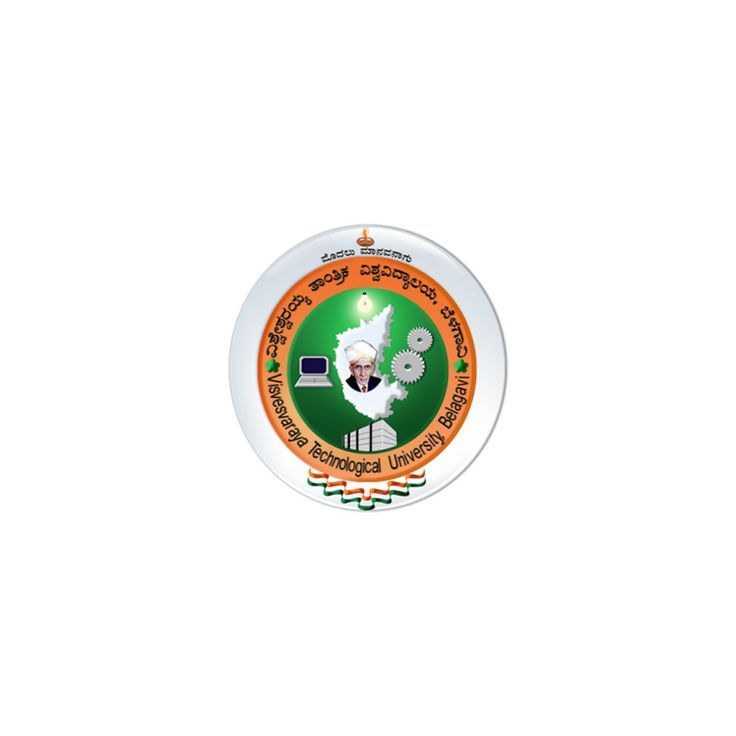
\includegraphics[width=2cm]{images/vtu_logo.jpg}\\[0.2cm]

{\color{darkblue}\textbf{\large Project Work Report}}\\
{\color{darkblue}\textbf{\large On}}\\[0.2cm]
{\color{darkred}\textbf{\Large ``AI-Powered Smart Glasses Using ESP32-CAM''}}\\[0.2cm]
{\small A report submitted in partial fulfilment of the requirements for}\\[0.1cm]
\textbf{PROJECT WORK}\\
{\small In}\\
{\color{darkred}\textbf{Computer Science and Engineering (IoT, CyberSecurity including Blockchain)}}\\[0.3cm]
\textbf{Submitted by}\\[0.3cm]

\begin{tabular}{l r}
\textbf{ARYA B SHETTY} & \textbf{4AL23IC007} \\
\textbf{HARINAND J} & \textbf{4AL23IC012} \\
\textbf{KARTHIK P} & \textbf{4AL23IC016} \\
\textbf{PAVAN SN} & \textbf{4AL23IC033} \\
\end{tabular}\\[0.3cm]

{\color{darkred}\textbf{Under the Guidance of}}\\[0.1cm]
{\color{darkred}\textit{\textbf{Prof. Jyothibha R Chinchankar}}}\\
{\color{darkred}\textit{Assistant Professor}}\\[0.3cm]

% === COLLEGE LOGO ===

\includegraphics[width=2cm]{images/alvas_logo.jpeg}\\[0.2cm]

{\color{darkblue}\textbf{DEPT. OF Computer Science and Engineering (IoT and Cyber Security\\including Blockchain)}}\\
{\color{darkblue}\textbf{ALVA'S INSTITUTE OF ENGINEERING \& TECHNOLOGY MIJAR,}}\\
{\small (Unit of Alva's Education Foundation, Moodbidri)}\\
{\small Affiliated to Visvesvaraya Technological University, Belagavi, Approved by AICTE,}\\
{\small New Delhi, Recognized by the Government of Karnataka.}\\
\textbf{Accredited by NAAC with A+ Grade}\\
{\small Shobavana Campus, Mijar, Moodbidri, D.K., Karnataka 2025-2026}
\end{center}
\newpage

% =================== CERTIFICATE ===================
\thispagestyle{empty}
\begin{center}
{\color{darkblue}\textbf{\large ALVA'S INSTITUTE OF ENGINEERING AND}}\\
{\color{darkblue}\textbf{\large TECHNOLOGY MIJAR, MOODBIDRI, D.K. -- 574225}}\\[0.5cm]

% === COLLEGE LOGO ===

\includegraphics[width=2.5cm]{images/alvas_logo.jpeg}\\[0.3cm]

{\color{darkblue}\textbf{DEPT. OF Computer Science and Engineering (IoT and Cyber Security\\including Blockchain)}}\\[0.5cm]
\textbf{\Large CERTIFICATE}\\[0.5cm]
\end{center}

This is to certify that the PROJECT entitled {\color{darkred}\textbf{``AI-POWERED SMART GLASSES USING ESP32-CAM''}} has been carried out by

\begin{center}
\begin{tabular}{l r}
ARYA B SHETTY & 4AL23IC007 \\
HARINAND J & 4AL23IC012 \\
KARTHIK P & 4AL23IC016 \\
PAVAN SN & 4AL23IC033 \\
\end{tabular}
\end{center}

The Bonafide students of the {\color{darkblue}Department of Computer Science and Engineering (IoT and Cyber Security including Blockchain)}, Alva's Institute of Engineering and Technology in {\color{darkred}\textbf{Department of Computer Science and Engineering (IoT and Cyber Security including Blockchain)}} of the \textbf{VISVESVARAYA TECHNOLOGICAL UNIVERSITY}, \textbf{BELAGAVI} during the year 2025--2026. It is certified that all corrections/suggestions indicated for Internal Assessment have been incorporated in the report deposited in the departmental library. The Project report has been approved as it satisfies the academic requirements concerning the Project prescribed for the Bachelor of Engineering Degree.

\vspace{2.5cm}
\noindent
\begin{tabular}{p{4.5cm}p{4cm}p{4.5cm}}
\centering\hrulefill & \centering\hrulefill & \centering\hrulefill \tabularnewline
\centering\small{\color{darkred}\textbf{Prof. Jyothibha R Chinchankar}} & \centering\small{\color{darkgreen}\textbf{Prof. Savitha SK}} & \centering\small{\color{darkblue}\textbf{Prof. Vasudev Shahapur}} \tabularnewline
\centering\small\textit{Project Guide} & \centering\small\textit{Project Coordinator} & \centering\small\textit{HOD, Dept. of CS(ICB)} \tabularnewline
\end{tabular}
\newpage

% =================== DECLARATION ===================
\thispagestyle{empty}
\begin{center}
{\color{darkblue}\textbf{\large ALVA'S INSTITUTE OF ENGINEERING AND}}\\
{\color{darkblue}\textbf{\large TECHNOLOGY MIJAR, MOODBIDRI D.K. -- 574225}}\\[0.5cm]

% === COLLEGE LOGO ===

\includegraphics[width=2.5cm]{images/alvas_logo.jpeg}\\[0.3cm]

{\color{darkgreen}\textbf{DEPARTMENT OF COMPUTER SCIENCE AND ENGINEERING}}\\
{\color{darkgreen}\textbf{(IoT AND CYBER SECURITY INCLUDING BLOCKCHAIN)}}\\[0.5cm]
\textbf{\Large \uline{DECLARATION}}\\[0.5cm]
\end{center}

We,\\
\hspace{1cm}\textbf{ARYA B SHETTY}\\
\hspace{1cm}\textbf{HARINAND J}\\
\hspace{1cm}\textbf{KARTHIK P}\\
\hspace{1cm}\textbf{PAVAN SN}\\[0.5cm]

Here by declare that the dissertation entitled, {\color{darkred}\textbf{AI-POWERED SMART GLASSES USING ESP32-CAM}} is being carried out by us under the supervision of our guide \textbf{Prof. Jyothibha R Chinchankar}, Assistant Professor, {\color{darkblue}Department of Computer Science and Engineering (IoT and Cyber Security including Blockchain)}, {\color{darkblue}Alva's Institute of Engineering and Technology, Moodbidri}, \textbf{DEPARTMENT OF COMPUTER SCIENCE AND ENGINEERING (IOT AND CYBER SECURITY INCLUDING BLOCKCHAIN)} of the \textbf{VISVESVARAYA TECHNOLOGICAL UNIVERSITY, BELAGAVI} during the academic year 2025--2026. The project is original and it has not been submitted for any other degree in any university.

\vspace{2cm}
\begin{center}
\begin{tabular}{l r}
ARYA B SHETTY & 4AL23IC007 \\
HARINAND J & 4AL23IC012 \\
KARTHIK P & 4AL23IC016 \\
PAVAN SN & 4AL23IC033 \\
\end{tabular}
\end{center}
\newpage

% =================== ACKNOWLEDGEMENT ===================
\thispagestyle{empty}
\begin{center}
\textbf{\Large ACKNOWLEDGEMENT}\\[0.5cm]
\end{center}

The satisfaction and euphoria that accompany a successful completion of any task would be incomplete without the mention of the people who made it possible. Success is the epitome of hard work and perseverance, but steadfast of all is encouraging guidance.

\vspace{0.5cm}
So, with gratitude, we acknowledge all those whose guidance and encouragement served as a beacon of light and crowned the effort with success.

\vspace{0.5cm}
The selection of this project work as well as the timely completion is mainly due to the interest and persuasion of our project guide \textbf{Prof. Jyothibha R Chinchankar}, Assistant Professor, \textbf{Department of Computer Science and Engineering (IoT and Cyber Security including Blockchain)}. We will remember her contribution forever.

\vspace{0.5cm}
We sincerely thank, \textbf{Dr. Vasudev Shahapur S}, Associate Professor and Head of the \textbf{Department of Computer Science and Engineering (IoT and Cyber Security including Blockchain)}, who has been the constant driving force behind the completion of the project.

\vspace{0.5cm}
We thank our beloved Principal, \textbf{Dr. Peter Fernandes}, for his constant help and support throughout.

\vspace{0.5cm}
We are indebted to the \textbf{Management of Alva's Institute of Engineering and Technology, Mijar, Moodbidri} for providing an environment that helped us in completing our project.

\vspace{0.5cm}
Also, we thank all the teaching and non-teaching staff of the Department of Computer Science and Engineering for the help rendered.

\vspace{2cm}
\begin{center}
\begin{tabular}{l r}
ARYA B SHETTY & 4AL23IC007 \\
HARINAND J & 4AL23IC012 \\
KARTHIK P & 4AL23IC016 \\
PAVAN SN & 4AL23IC033 \\
\end{tabular}
\end{center}
\newpage

% =================== ABSTRACT ===================
\thispagestyle{empty}
\begin{center}
\textbf{\Large ABSTRACT}\\[0.5cm]
\end{center}

The proliferation of Artificial Intelligence and Internet of Things technologies has created unprecedented opportunities for developing intelligent wearable devices that can augment human perception. Visually impaired individuals, numbering over 2.2 billion globally according to the World Health Organization, face significant challenges in understanding and navigating their physical environment. While commercial smart glasses from companies such as Google and Meta offer some degree of visual assistance, their prohibitive pricing places them beyond the reach of most users, particularly in developing nations. This project proposes the design and implementation of AI-powered smart glasses that will address this accessibility gap by leveraging affordable hardware and free-tier cloud AI services.

\vspace{0.3cm}
The system will be built around the ESP32-CAM microcontroller, a compact and low-cost development board featuring a dual-core Xtensa LX6 processor, integrated Wi-Fi connectivity, and an onboard OV2640 2-megapixel camera module. Additional hardware components will include an SSD1306 OLED display for visual output, an INMP441 I2S digital MEMS microphone for voice input, a micro speaker for text-to-speech audio feedback, and two push buttons for mode selection. The entire assembly will be designed to be mounted on a standard glasses frame, creating a lightweight and portable wearable device.

\vspace{0.3cm}
The software architecture will employ a hybrid cloud-local processing model. Computationally intensive AI tasks such as image description and question answering will be offloaded to cloud-based large language models (Llama 4 Scout 17B for multimodal vision tasks, Llama 3.3 70B Versatile for natural language processing) accessed via the Groq free-tier API, which provides up to 14,400 free API calls per day. Lightweight tasks such as optical character recognition and speech-to-text transcription will be processed locally using EasyOCR and OpenAI Whisper-tiny respectively, enabling offline functionality for these capabilities.

\vspace{0.3cm}
The backend server will be built using Python Flask and will implement a novel Smart Routing architecture that serves as the core technical contribution of this project. The Smart Router will intelligently distribute incoming AI requests across cloud and local processing pathways while managing model lifecycle to optimize memory usage. It will ensure that only one local AI model is loaded into GPU memory at any given time, with explicit model unloading after each request through Python garbage collection and PyTorch CUDA cache clearing. This memory management strategy is expected to keep peak RAM usage under 600 MB, making the system compatible with entry-level consumer GPUs.

\vspace{0.3cm}
The system will be designed to provide five core AI capabilities: (1) scene description, where the camera captures an image and the AI generates a detailed textual description; (2) text extraction via OCR, enabling the user to read text from signs, books, and labels; (3) speech-to-text transcription for voice command recognition; (4) question answering, allowing the user to ask contextual questions; and (5) language translation between supported languages. All AI tasks are expected to achieve response times under 2 seconds, providing near-real-time assistance. The hardware prototype will use readily available, low-cost components, making it a practical and affordable assistive technology solution for visually impaired individuals in developing countries.

\vspace{0.3cm}
\textbf{Keywords:} Smart Glasses, ESP32-CAM, Artificial Intelligence, Computer Vision, IoT, Groq API, Flask, EasyOCR, Whisper, Assistive Technology, Smart Routing, Edge Computing, Wearable Technology, Embedded Systems.
\newpage

% =================== TABLE OF CONTENTS ===================
% =====================================================================
% TABLE OF CONTENTS (Manual Tabular Format)
% =====================================================================
\thispagestyle{empty}
\begin{center}
\textbf{\Large TABLE OF CONTENTS}\\[0.5cm]
\end{center}

\begin{longtable}{|c|p{9cm}|c|}
\hline
\textbf{SL. NO.} & \textbf{TITLE} & \textbf{PAGE NO.} \\
\hline
\endfirsthead
\hline
\textbf{SL. NO.} & \textbf{TITLE} & \textbf{PAGE NO.} \\
\hline
\endhead
1 & INTRODUCTION & 1 \\
1.1 & \quad Overview & \\
1.2 & \quad Purpose & \\
1.3 & \quad Project Relevance & \\
\hline
2 & LITERATURE SURVEY & 4 \\
2.1 & \quad Low-Cost Smart Glasses using ESP32 & \\
2.2 & \quad AI-Powered Smart Glasses for the Blind & \\
2.3 & \quad Deep Learning-Based Smart Glasses & \\
2.4 & \quad Speech Recognition for Wearable Devices & \\
2.5 & \quad Large Language Models for Visual Understanding & \\
2.6 & \quad Optical Character Recognition for Accessibility & \\
2.7 & \quad Edge Computing for AI Applications & \\
2.8 & \quad Research Gap & \\
\hline
3 & PROBLEM STATEMENT AND OBJECTIVES & 8 \\
3.1 & \quad Problem Statement & \\
3.2 & \quad Objectives & \\
\hline
4 & SYSTEM REQUIREMENTS AND SPECIFICATION & 10 \\
4.1 & \quad Hardware Requirements & \\
4.1.1 & \qquad Microcontroller -- ESP32-CAM & \\
4.1.2 & \qquad Display Module -- SSD1306 OLED & \\
4.1.3 & \qquad Microphone -- INMP441 & \\
4.1.4 & \qquad Camera Module -- OV2640 & \\
4.1.5 & \qquad Audio Output -- Micro Speaker & \\
4.1.6 & \qquad Input Controls -- Push Buttons & \\
4.1.7 & \qquad Power Supply & \\
4.2 & \quad Software Requirements & \\
4.2.1 & \qquad Programming Languages & \\
4.2.2 & \qquad Frameworks and Libraries & \\
4.2.3 & \qquad Communication Protocols & \\
4.3 & \quad Power Requirements & \\
\hline
5 & PROPOSED METHODOLOGY & 14 \\
5.1 & \quad Software Development & \\
5.1.1 & \qquad Control Code Development & \\
5.1.2 & \qquad Smart Routing Architecture & \\
5.2 & \quad Data Flow Pipeline & \\
5.3 & \quad Testing Plan & \\
\hline
6 & SYSTEM ARCHITECTURE & 18 \\
6.1 & \quad System Block Diagram & \\
6.2 & \quad Power Supply Subsystem & \\
6.3 & \quad ESP32 Control Unit & \\
6.4 & \quad Sensor Subsystem & \\
6.5 & \quad OLED Display Subsystem & \\
6.6 & \quad Flask Web Server (Smart Router) & \\
\hline
7 & EXPECTED OUTCOME & 22 \\
7.1 & \quad Functional Outcomes & \\
7.2 & \quad Expected Performance Metrics & \\
7.3 & \quad System-Level Performance Expectations & \\
\hline
8 & ADVANTAGES AND FUTURE SCOPE & 24 \\
8.1 & \quad Advantages & \\
8.2 & \quad Future Scope & \\
\hline
9 & CONCLUSION & 27 \\
\hline
10 & REFERENCES & 28 \\
\hline
\end{longtable}
\newpage

\disableborder

% ================================================================
%                    CHAPTERS (with header/footer)
% ================================================================
\pagestyle{chapterpages}
\setcounter{page}{1}
% =====================================================================
% CHAPTER 1: INTRODUCTION
% =====================================================================
\chapter{Introduction}

\section{Overview}
The rapid advancement of Artificial Intelligence and embedded systems has opened new frontiers in wearable technology. Smart glasses represent one of the most promising applications at the intersection of these technologies, offering the potential to augment human perception through real-time computational assistance. This project will present the design and implementation of AI-powered smart glasses that leverage the ESP32-CAM microcontroller as the primary hardware platform, combined with a hybrid cloud-local AI backend architecture to deliver sophisticated visual and linguistic assistance capabilities.

The ESP32-CAM is a compact, low-cost development board featuring a dual-core Xtensa LX6 processor running at 240 MHz with 520 KB of SRAM and 4 MB of flash memory. The module includes an integrated OV2640 camera capable of capturing images at resolutions up to 1600$\times$1200 pixels. For this project, images will be captured at 640$\times$480 (VGA) resolution to balance quality with transmission speed over wireless networks. The ESP32-CAM supports IEEE 802.11 b/g/n Wi-Fi and Bluetooth 4.2, enabling seamless wireless communication with the backend server running on a local machine.

The backend server will implement a novel Smart Routing architecture that intelligently distributes incoming AI tasks across multiple processing pathways. Computationally intensive tasks such as image understanding and natural language question answering will be offloaded to cloud-based large language models accessed through the Groq API free tier. This tier provides access to state-of-the-art models including Llama 4 Scout 17B for multimodal vision tasks and Llama 3.3 70B Versatile for language processing, with a generous allowance of 14,400 free API calls per day. These cloud-based models will enable the system to perform advanced reasoning, scene understanding, and multilingual translation without imposing any computational burden on the local hardware.

Lightweight tasks that benefit from low latency and offline capability will be processed locally using open-source AI models. EasyOCR will handle optical character recognition for extracting text from images, supporting over 80 languages with robust accuracy. OpenAI Whisper in its tiny configuration (39 million parameters) will provide speech-to-text transcription capability with minimal resource requirements. The Smart Router will ensure that only one local model occupies memory at any given time, and models will be explicitly unloaded after each request. This memory management strategy is expected to keep peak RAM usage under 600 MB, making the system compatible with entry-level NVIDIA GPUs such as the GTX 1650 and RTX 3050.

The integration of multiple AI modalities within a single wearable device represents a significant step forward in affordable assistive technology. By combining computer vision, natural language processing, optical character recognition, and automatic speech recognition, the system will provide comprehensive assistance that goes far beyond what traditional assistive devices such as white canes or basic electronic travel aids can offer.

\section{Purpose}
The primary purpose of this project is to develop an affordable, functional smart glasses prototype that demonstrates the practical application of AI-powered assistive technology. The project will aim to bridge the gap between expensive commercial smart glasses and the needs of users who require visual assistance, particularly visually impaired individuals in developing countries where cost is a significant barrier to adoption.

Commercial smart glasses such as Google Glass Enterprise Edition and Meta Ray-Ban Smart Glasses are priced well beyond the reach of most users in India and other developing nations. By utilizing the ESP32-CAM platform and free-tier cloud AI services, this project will demonstrate that comparable AI capabilities can be delivered at a fraction of the cost using readily available components. The system will provide five core functionalities---scene description, text extraction, speech recognition, question answering, and translation---all accessible through a simple button-based interface mounted on a standard glasses frame.

The project will also serve as a proof-of-concept for the hybrid cloud-local AI architecture, demonstrating that sophisticated AI workloads can be efficiently distributed between cloud and edge resources without requiring expensive dedicated hardware or paid cloud subscriptions. This architectural pattern will have broader implications for IoT device design, as it enables resource-constrained edge devices to access powerful AI capabilities while maintaining low latency for time-critical operations.

Furthermore, the project will contribute to the field of accessible technology by providing an open-source, replicable design that can be adopted and customized by researchers, educators, and humanitarian organizations working to improve the lives of visually impaired individuals. The use of open-source software components and widely available hardware ensures that the design will be accessible to a broad audience.

\section{Project Relevance}
This project is relevant to multiple domains within computer science and engineering, reflecting the interdisciplinary nature of modern IoT and AI applications:

\begin{itemize}[leftmargin=1.5cm]
\item \textbf{Internet of Things (IoT):} The system will demonstrate core IoT principles through wireless sensor data collection (camera, microphone), cloud processing via RESTful APIs, and actuator feedback through the OLED display and speaker. The ESP32-CAM will serve as an IoT edge node that communicates with a local gateway server.

\item \textbf{Embedded Systems:} The ESP32-CAM firmware development will involve real-time programming, peripheral management (camera, I2C for OLED, I2S for microphone), interrupt-driven button handling, and resource-constrained optimization. The firmware will need to manage multiple communication protocols simultaneously while maintaining responsiveness.

\item \textbf{Artificial Intelligence:} The project will integrate multiple AI paradigms including computer vision (scene understanding via multimodal LLMs), natural language processing (question answering and translation), optical character recognition (text extraction from images), and automatic speech recognition (voice-to-text transcription). The Smart Routing architecture will demonstrate practical AI model lifecycle management.

\item \textbf{Cloud Computing:} The hybrid architecture will demonstrate practical cloud-edge computing patterns, RESTful API integration, and intelligent workload distribution strategies. The use of the Groq API free tier will showcase how cloud AI services can be leveraged cost-effectively for resource-constrained applications.

\item \textbf{Assistive Technology:} The system will directly address the needs of visually impaired users, aligning with the United Nations Sustainable Development Goal 10 (Reduced Inequalities) and Goal 3 (Good Health and Well-being). The dual output modality (visual display and audio speaker) will ensure accessibility for users with varying degrees of visual impairment.

\item \textbf{Cybersecurity and Privacy:} The edge-processing approach for sensitive tasks (OCR, speech) will keep personal data local, while cloud API calls will transmit only encoded image data over HTTPS-encrypted channels. This privacy-aware architecture will demonstrate responsible AI deployment practices in wearable devices.
\end{itemize}

% =====================================================================
% CHAPTER 2: LITERATURE SURVEY
% =====================================================================
\chapter{Literature Survey}

A comprehensive review of existing literature and related work has been conducted to understand the current state of smart glasses technology, identify key advancements in the field, and determine the research gaps that this project will aim to address. The following subsections present a critical analysis of seven significant works that form the foundation for the proposed system design.

\section{Low-Cost Smart Glasses using ESP32}
Das, Saxena, and Rout (2021) presented a low-cost smart glass implementation using the ESP-32 microcontroller at the IEEE 2nd International Conference on Applied Electromagnetics, Signal Processing, and Communication (AESPC). Their work demonstrated the feasibility of building wearable visual assistance devices using affordable microcontroller platforms. The system employed the ESP32 for basic image capture and wireless transmission, establishing that the platform possesses sufficient computational resources for real-time image acquisition and Wi-Fi communication. However, their implementation was limited to basic image capture and display without any AI-powered analysis capabilities. The system lacked scene understanding, text extraction, or any form of natural language interaction, rendering it a passive data collection device rather than an intelligent assistive tool. The proposed project will extend this foundational approach by adding a comprehensive AI processing pipeline with both cloud and local model integration.

\section{AI-Powered Smart Glasses for the Blind}
Ramesh Babu et al. (2025) proposed AI-powered smart glasses for visually impaired users using OpenCV and Python at the IEEE Wireless Antenna and Microwave Symposium (WAMS). Their system focused on real-time object detection using traditional computer vision techniques, specifically employing Haar cascades and HOG (Histogram of Oriented Gradients) descriptors for feature extraction. While effective for basic object identification tasks such as face detection and pedestrian recognition, their approach lacked the ability to provide natural language descriptions of scenes or answer contextual questions about the visual environment. The system could identify \textit{what} objects were present but could not explain \textit{what was happening} in the scene or respond to user queries. The proposed project will address this limitation by incorporating large language models capable of generating detailed, context-aware descriptions and engaging in conversational question answering about captured scenes.

\section{Deep Learning-Based Smart Glasses}
Lin et al. (2020) developed a smart glasses application system for visually impaired people based on deep learning at the Indo-Taiwan 2nd International Conference on Computing, Analytics and Networks (Indo-Taiwan ICAN). Their work employed convolutional neural networks (CNNs) for object classification, achieving high accuracy on standard benchmarks. However, their system required a powerful GPU-equipped computer with dedicated VRAM exceeding 8 GB for real-time inference, significantly limiting its portability and accessibility. The computational requirements meant that the system could only function in controlled environments with access to high-performance hardware. The proposed hybrid cloud-local architecture will overcome this constraint by offloading heavy AI tasks to free cloud APIs while keeping the local compute requirements to a minimum, enabling operation on consumer-grade hardware.

\section{Speech Recognition for Wearable Devices}
Radford et al. (2023) introduced Whisper, a robust speech recognition system trained on 680,000 hours of multilingual and multitask supervised audio data, at the 40th International Conference on Machine Learning (ICML). The Whisper model family ranges from tiny (39 million parameters, approximately 145 MB) to large (1.5 billion parameters, approximately 3 GB), offering a spectrum of accuracy-efficiency tradeoffs suitable for different deployment scenarios. The tiny model, despite its compact size, achieves competitive word error rates on standard benchmarks such as LibriSpeech and Common Voice. The proposed project will utilize the Whisper-tiny model for voice command recognition, as it provides an optimal balance between accuracy and resource consumption for the target deployment environment. The model's ability to function with minimal GPU memory will complement the Smart Routing architecture's memory management strategy.

\section{Large Language Models for Visual Understanding}
Touvron et al. (2023) published the Llama 2 family of open foundation and fine-tuned chat models from Meta AI Research. These models demonstrated that open-source large language models could achieve performance competitive with proprietary systems such as GPT-3.5 and PaLM across a wide range of natural language understanding and generation tasks. The subsequent Llama 3.3 and Llama 4 Scout models, which the proposed project will utilize through the Groq API, represent significant improvements in both language understanding and multimodal reasoning capabilities. Llama 4 Scout 17B, in particular, introduces native multimodal processing that can accept both text and image inputs, making it ideal for scene description tasks. The availability of these models through free-tier cloud APIs fundamentally changes the economics of AI-powered wearable devices.

\section{Optical Character Recognition for Accessibility}
JaidedAI (2020) developed EasyOCR, an open-source optical character recognition library supporting over 80 languages including English, Hindi, Kannada, and other Indian regional scripts. Unlike commercial OCR solutions that require paid subscriptions or API access, EasyOCR is freely available under the Apache 2.0 license and can run entirely on local hardware with modest memory requirements of approximately 180 MB. The library uses a combination of CRAFT (Character Region Awareness for Text detection) for text region detection and deep learning-based recognition networks for character identification. The recognition pipeline supports multiple scripts simultaneously and handles curved, rotated, and partially occluded text with reasonable accuracy. The proposed project will leverage EasyOCR for the text extraction capability, enabling the smart glasses to read text from signs, books, documents, and product labels---a critical feature for visually impaired users navigating public spaces.

\section{Edge Computing for AI Applications}
Chen and Ran (2019) provided a comprehensive review of deep learning with edge computing in the Proceedings of the IEEE, examining the challenges and opportunities of deploying AI models on resource-constrained edge devices. Their survey highlighted the importance of distributing AI workloads between cloud and edge devices to achieve optimal latency (sub-second response times for real-time applications), bandwidth utilization (reducing data transmission by processing locally where possible), and privacy (keeping sensitive data on-device). They identified model partitioning and workload scheduling as key technical challenges that remain actively researched. The proposed project's Smart Routing architecture will directly implement the principles outlined in their survey, demonstrating a practical application of cloud-edge AI distribution in a wearable device context with intelligent model lifecycle management.

\section{Research Gap}
The literature review reveals that while several smart glasses projects exist in the academic and commercial domains, most suffer from one or more of the following critical limitations:

\begin{enumerate}[leftmargin=1.5cm]
\item \textbf{High Cost:} Commercial solutions are priced beyond the reach of users in developing countries, and academic prototypes often use expensive hardware platforms such as Raspberry Pi 4 with dedicated GPUs.

\item \textbf{Heavy Computational Requirements:} Existing AI-powered smart glasses require high-performance GPUs with 8--12 GB of VRAM for local inference, making them incompatible with consumer-grade hardware.

\item \textbf{Limited AI Capabilities:} Most academic prototypes are restricted to a single AI modality---either object detection, or OCR, or speech recognition---without providing an integrated multi-modal experience.

\item \textbf{No Memory Optimization:} None of the reviewed works address the challenge of running multiple AI models efficiently on resource-constrained hardware through intelligent model lifecycle management.
\end{enumerate}

This project will address all four limitations through its affordable hardware design based on the ESP32-CAM, hybrid cloud-local AI architecture utilizing free-tier APIs, comprehensive multi-modal AI capabilities spanning five distinct functions, and the novel Smart Routing memory management system that will enable operation on entry-level consumer hardware.

% =====================================================================
% CHAPTER 3: PROBLEM STATEMENT AND OBJECTIVES
% =====================================================================
\chapter{Problem Statement and Objectives}

\section{Problem Statement}
Visually impaired individuals face significant challenges in understanding and navigating their physical environment. While assistive devices such as white canes and guide dogs provide basic obstacle avoidance, they are fundamentally unable to offer visual understanding capabilities such as reading text from signs, identifying objects in a scene, or answering contextual questions about the surroundings. Modern AI technologies possess these capabilities with remarkable accuracy, but deploying them in a wearable form factor for widespread use presents three critical challenges:

\begin{enumerate}[leftmargin=1.5cm]
\item \textbf{Cost Barrier to Adoption:} Commercial smart glasses with AI capabilities, such as Google Glass Enterprise Edition and Meta Ray-Ban Smart Glasses, are prohibitively expensive for the majority of users, especially in developing countries like India where the average monthly income is significantly lower than in Western nations. This economic barrier effectively excludes the most vulnerable populations---those who could benefit most from AI-powered visual assistance---from accessing this technology. No affordable alternative currently exists that provides comprehensive AI-based scene understanding, text reading, and conversational interaction through a wearable device.

\item \textbf{Computational Resource Requirements:} State-of-the-art AI vision models such as GPT-4 Vision, LLaVA, and CLIP require powerful GPUs with 12+ GB of dedicated VRAM for local inference. Running these models on a user's personal laptop or any edge computing device without expensive hardware upgrades is impractical. Even smaller, optimized models like MobileNet and EfficientNet, while deployable on edge devices, lack the natural language understanding and generative capabilities needed for scene description and conversational question answering. This computational gap prevents the deployment of truly intelligent visual assistance on consumer hardware.

\item \textbf{Multi-Model Memory Management Complexity:} A comprehensive assistive system requires multiple AI models operating in concert---vision models for scene understanding, language models for question answering and translation, OCR models for text extraction, and speech recognition models for voice input. Running all these models simultaneously would require over 12 GB of combined GPU memory, far exceeding the capacity of most consumer-grade GPUs (4--8 GB). No existing framework or architecture addresses the challenge of running multiple heterogeneous AI models efficiently on resource-constrained hardware through intelligent scheduling and memory lifecycle management.
\end{enumerate}

There is a clear and urgent need for an affordable smart glasses solution that can deliver advanced, multi-modal AI capabilities using consumer-grade hardware and freely available cloud services, making AI-powered assistive technology accessible to users regardless of their economic background or technical expertise.

\section{Objectives}
The specific objectives of this project are defined as follows:

\begin{enumerate}[leftmargin=1.5cm]
\item \textbf{Hardware Prototype Design:} To design and fabricate a wearable smart glasses prototype using the ESP32-CAM microcontroller with OV2640 camera module, SSD1306 OLED display (128$\times$64, I2C), INMP441 I2S digital MEMS microphone, micro speaker (8 ohm, 0.5W), two push buttons for mode selection, and a rechargeable LiPo battery with TP4056 charging module and AMS1117-3.3V voltage regulator. The complete assembly will be mounted on a standard glasses frame for comfortable wearability.

\item \textbf{Hybrid AI Backend Development:} To develop a Flask-based backend server with a Smart Routing architecture that will intelligently distribute AI tasks between cloud-based models (Llama 4 Scout 17B for vision and Llama 3.3 70B Versatile for language processing, accessed via the Groq free-tier API) and locally-running open-source models (EasyOCR for optical character recognition and Whisper-tiny for speech-to-text transcription). The Smart Router will manage model loading, unloading, and memory lifecycle to optimize resource utilization.

\item \textbf{Multi-Modal AI Functionality:} To implement five core AI functionalities within the system: (a) scene description---generating natural language descriptions of captured images; (b) text extraction via OCR---reading printed text from signs, books, documents, and labels; (c) speech-to-text transcription---converting spoken voice commands to text; (d) question answering---providing AI-generated answers to user queries; and (e) language translation---translating text between supported languages.

\item \textbf{Performance Optimization:} To achieve response times under 2 seconds for all AI tasks while maintaining peak GPU memory usage below 600 MB through the Smart Routing memory management strategy. Cloud-based tasks will target sub-second response times, while local tasks will target response times under 2 seconds.

\item \textbf{Comprehensive System Testing:} To validate the system through comprehensive testing across three tiers: (a) AI model accuracy tests to verify correct functionality of each model independently; (b) memory management tests to confirm that the Smart Routing architecture maintains memory usage within target limits; and (c) Flask endpoint integration tests to verify correct HTTP request handling, response formatting, and error management.

\item \textbf{Dual-Output Accessibility:} To provide both text-to-speech audio output through the micro speaker and visual text output through the OLED display for delivering AI responses to the user, ensuring accessibility for users with varying degrees of visual impairment and accommodating different usage contexts (e.g., noisy environments where audio is impractical, or quiet environments where screen reading is preferred).
\end{enumerate}

% =====================================================================
% CHAPTER 4: SYSTEM REQUIREMENTS AND SPECIFICATION
% =====================================================================
\chapter{System Requirements and Specification}

\section{Hardware Requirements}

\subsection{Microcontroller -- ESP32-CAM}
The ESP32-CAM will serve as the central processing unit of the smart glasses. It is based on the ESP32-S module, featuring a dual-core Xtensa LX6 processor running at 240 MHz with 520 KB of SRAM and 4 MB of flash memory. The module includes an integrated OV2640 camera capable of capturing images at resolutions up to 1600$\times$1200 pixels. For this project, images will be captured at 640$\times$480 (VGA) resolution to balance image quality with wireless transmission speed. The ESP32-CAM supports IEEE 802.11 b/g/n Wi-Fi and Bluetooth 4.2, enabling wireless communication with the backend server. The module also includes a micro SD card slot for optional local storage of captured images and a built-in LED flash for low-light photography.

\subsection{Display Module -- SSD1306 OLED (0.96 inch, 128$\times$64, I2C)}
The SSD1306 OLED display is a compact, self-emitting display module with 128$\times$64 pixel resolution and a 0.96-inch diagonal screen size. It will communicate with the ESP32 via the I2C protocol using GPIO 14 (SDA) and GPIO 15 (SCL) pins. Two 4.7k ohm pull-up resistors will be required on the I2C data and clock lines to ensure reliable communication at 400 kHz. The display will be mounted on the glasses frame near the user's field of vision and will show AI-generated text responses. Its low power consumption (typically 20 mA at 3.3V) makes it suitable for battery-powered operation. The OLED technology provides high contrast ratio (10,000:1) and wide viewing angles (up to 160 degrees), ensuring readability in diverse lighting conditions.

\subsection{Microphone -- INMP441 I2S Digital MEMS}
The INMP441 is a high-precision digital MEMS (Micro-Electro-Mechanical Systems) microphone that will output audio data via the I2S (Inter-IC Sound) protocol. It provides a signal-to-noise ratio of 61 dB and a sensitivity of -26 dBFS, ensuring clear audio capture for speech recognition. The I2S interface provides superior audio quality compared to analog microphones by eliminating analog-to-digital conversion noise at the microphone interface. The microphone will capture the user's voice commands for speech-to-text processing by the Whisper-tiny model. The digital output format (24-bit, up to 48 kHz sampling rate) will ensure high-fidelity audio data for accurate transcription.

\subsection{Camera Module -- OV2640}
The OV2640 camera module is integrated into the ESP32-CAM board. It is a 2-megapixel CMOS image sensor capable of capturing images in JPEG, RGB565, and YUV422 formats. The camera supports automatic exposure control (AEC), automatic gain control (AGC), and automatic white balance (AWB), enabling consistent image quality across varying lighting conditions. For this project, JPEG format at VGA resolution will be used to minimize the data size (approximately 30--50 KB per frame) for efficient wireless transmission. The camera will interface with the ESP32 through an 8-bit parallel data bus with XCLK (20 MHz external clock), PCLK (pixel clock), VSYNC (vertical sync), and HREF (horizontal reference) timing signals.

\subsection{Audio Output -- Micro Speaker (8 ohm, 0.5W, 40mm)}
A miniature speaker with 8 ohm impedance and 0.5W power rating will provide audio output for text-to-speech feedback. The speaker's compact 40mm diameter and lightweight construction will make it suitable for integration into the glasses frame. This will allow the user to hear AI-generated responses without needing to look at the OLED display, providing hands-free and eyes-free operation that is particularly beneficial for visually impaired users.

\subsection{Input Controls -- Push Buttons ($\times$2)}
Two momentary tactile push buttons will provide user input for mode selection and action triggering. Each button will be connected with a 10k ohm pull-up resistor to ensure clean digital signal transitions and prevent floating input states. Software debouncing with a 200ms delay will be implemented in the ESP32 firmware to prevent multiple triggers from a single press. Button 1 will cycle through the five operating modes (Scene, OCR, Voice, Q\&A, Translate), while Button 2 will trigger the active function (capture image or start recording).

\subsection{Power Supply -- LiPo Battery + TP4056 + AMS1117}
The system will be powered by a 3.7V, 1000 mAh lithium polymer rechargeable battery with a TP4056 USB micro charging module and an AMS1117-3.3V linear voltage regulator. The TP4056 will provide safe lithium battery charging with automatic cutoff at 4.2V and undervoltage protection at 2.5V. The AMS1117 regulator will convert the battery voltage (3.0V--4.2V across the discharge curve) to a stable 3.3V output required by all system components. Two 100nF ceramic decoupling capacitors will be placed near the voltage regulator output and the ESP32 power input pins to filter high-frequency noise and prevent brownout resets during Wi-Fi transmission bursts.

\subsection{Supporting Components}
Additional components will include resistors (4.7k ohm $\times$2 for I2C pull-ups on SDA and SCL lines, 10k ohm $\times$2 for button pull-ups), ceramic capacitors (100nF $\times$2 for power supply decoupling), a set of jumper wires for interconnections, and a standard glasses frame for mounting all electronic components. The glasses frame will be selected to accommodate the ESP32-CAM module, display, microphone, speaker, buttons, and battery in a comfortable and balanced configuration.

\vspace{0.5cm}
\noindent The hardware components listed above are readily available from standard electronics suppliers and online marketplaces, making the prototype accessible and reproducible for academic and research purposes.

\section{Software Requirements}

\subsection{Programming Languages}
\begin{itemize}[leftmargin=1.5cm]
\item \textbf{Python 3.10+:} Will serve as the primary language for the Flask backend server, AI model integration, Smart Routing logic, memory management, and API client operations. Python's extensive ecosystem of AI/ML libraries (PyTorch, EasyOCR, Whisper) and web frameworks (Flask) makes it the ideal choice for the backend development.

\item \textbf{C/C++ (Arduino Framework):} Will be used for ESP32-CAM firmware development within the Arduino IDE 2.x environment. The firmware will handle camera initialization, Wi-Fi connectivity, HTTP POST request construction, I2C display communication (using Adafruit SSD1306 library), I2S microphone data acquisition, GPIO interrupt handling for buttons, and JSON response parsing.
\end{itemize}

\subsection{Frameworks and Libraries}
\begin{itemize}[leftmargin=1.5cm]
\item \textbf{Flask 3.0+:} A lightweight Python web framework that will implement the Smart Router backend with RESTful API endpoints for each of the five AI capabilities. Flask's minimal overhead and extensibility make it suitable for the single-server deployment model.

\item \textbf{Groq Python SDK (v1.2):} The official client library for accessing the Groq cloud API. It will provide programmatic access to Llama 4 Scout 17B (multimodal vision model for scene description) and Llama 3.3 70B Versatile (language model for question answering, translation, and text generation).

\item \textbf{EasyOCR 1.7+:} An open-source optical character recognition library supporting 80+ languages. It will run locally on the backend server for text extraction from captured images, using a combination of CRAFT text detection and deep learning-based character recognition.

\item \textbf{OpenAI Whisper (tiny model):} An open-source speech recognition model with 39 million parameters and approximately 145 MB memory footprint. It will provide local speech-to-text transcription capability for voice command processing.

\item \textbf{PyTorch 2.0+:} The deep learning framework that will provide the inference runtime environment for both EasyOCR and Whisper models, including CUDA GPU acceleration support and memory management utilities.

\item \textbf{psutil:} A cross-platform system monitoring library that will track RAM, CPU, and GPU usage during operation, enabling the Smart Router to make informed decisions about model loading and unloading.

\item \textbf{python-dotenv:} A library for managing environment variables and API keys securely through \texttt{.env} files, ensuring that sensitive credentials are not hardcoded in the source code.
\end{itemize}

\subsection{Communication Protocols}
\begin{itemize}[leftmargin=1.5cm]
\item \textbf{HTTP/REST:} The ESP32-CAM will communicate with the Flask backend via HTTP POST requests carrying Base64-encoded image or audio data in JSON format. The server will respond with JSON payloads containing the AI-generated text response, processing time, and status information.

\item \textbf{I2C (Inter-Integrated Circuit):} A two-wire serial protocol that will connect the ESP32 to the SSD1306 OLED display at device address 0x3C with 400 kHz clock speed. The I2C bus requires two signal lines: SDA (Serial Data) and SCL (Serial Clock), each with 4.7k ohm pull-up resistors.

\item \textbf{I2S (Inter-IC Sound):} A three-wire digital audio protocol that will connect the INMP441 microphone to the ESP32 for high-quality audio data transfer. The I2S interface uses WS (Word Select), SCK (Serial Clock), and SD (Serial Data) signals.

\item \textbf{Wi-Fi (IEEE 802.11 b/g/n):} The primary wireless networking protocol enabling communication between the ESP32-CAM and the backend server over the local area network. The ESP32 will operate in station (STA) mode, connecting to an existing Wi-Fi access point.

\item \textbf{HTTPS (for Cloud API):} The Groq API communication from the Flask backend will use HTTPS (TLS 1.2+) for secure, encrypted transmission of image data and AI model responses between the local server and the Groq cloud infrastructure.
\end{itemize}

\section{Power Requirements}
The system will operate on a 3.7V lithium polymer battery with the following estimated power budget:

\begin{table}[h]
\centering
\begin{tabular}{|l|c|c|}
\hline
\textbf{Component} & \textbf{Current Draw} & \textbf{Voltage} \\
\hline
ESP32-CAM (active with Wi-Fi) & 160--260 mA & 3.3V \\
SSD1306 OLED Display & 20 mA & 3.3V \\
INMP441 Microphone & 1.4 mA & 3.3V \\
Micro Speaker (during playback) & 60 mA & 3.3V \\
TP4056 + AMS1117 quiescent & 5 mA & 3.7V \\
\hline
\textbf{Total Peak Consumption} & \textbf{$\approx$346 mA} & \textbf{3.3V} \\
\hline
\end{tabular}
\caption{Estimated Power Consumption Budget}
\end{table}

With a 1000 mAh battery, the system is expected to provide approximately 2.5--3 hours of continuous active use. In practical intermittent usage scenarios (where the system is idle between user commands), battery life is expected to extend to approximately 4--5 hours. The TP4056 module will enable convenient USB micro charging, supporting charge rates up to 1A for a full charge in approximately 1--1.5 hours.

% =====================================================================
% CHAPTER 5: PROPOSED METHODOLOGY
% =====================================================================
\chapter{Proposed Methodology}

\section{Software Development}

\subsection{Control Code Development}
The software architecture will follow a client-server model with the ESP32-CAM acting as the client and the Flask application serving as the backend server. The development process will involve two parallel tracks that will be integrated during the system integration phase.

\subsubsection*{ESP32-CAM Firmware (C++/Arduino)}
The firmware will be developed using the Arduino IDE 2.x with the ESP32 board support package. The firmware will initialize the camera module in JPEG mode at VGA (640$\times$480) resolution, establish Wi-Fi connectivity with the local network using stored SSID and password credentials, and enter a main loop that monitors button inputs via GPIO interrupt handlers.

When the user presses the action button (Button 2), the firmware will execute the following sequence based on the currently selected mode:

\begin{enumerate}[leftmargin=1.5cm]
\item \textbf{Image Capture Mode:} The firmware will capture a single image frame from the OV2640 camera buffer, encode the JPEG data in Base64 format using an embedded Base64 encoding library, construct an HTTP POST request with a JSON payload containing the encoded image and the request type identifier, and transmit it to the Flask server's corresponding endpoint. The total payload size will be approximately 40--70 KB after Base64 encoding.

\item \textbf{Audio Capture Mode:} For speech-to-text functionality, the firmware will sample audio from the INMP441 microphone via the I2S peripheral at 16 kHz sample rate with 16-bit resolution. Audio data will be buffered for a configurable duration (default 5 seconds), then Base64-encoded and transmitted to the \texttt{/transcribe} endpoint.
\end{enumerate}

Upon receiving the JSON response from the server, the firmware will extract the AI-generated text field and render it on the SSD1306 OLED display using the Adafruit SSD1306 and Adafruit GFX libraries. For text responses exceeding the 8-line display capacity, automatic vertical scrolling will be implemented. The response text will also be available for text-to-speech output through the micro speaker.

The mode selection button (Button 1) will cycle through the five operating modes in sequence: Scene Description $\rightarrow$ OCR $\rightarrow$ Voice $\rightarrow$ Q\&A $\rightarrow$ Translate. The current mode will be displayed as a status indicator on the OLED screen.

\subsubsection*{Flask Backend Server (Python)}
The backend will implement five RESTful API endpoints corresponding to the five AI capabilities:

\begin{itemize}[leftmargin=1.5cm]
\item \texttt{POST /analyze-image} --- Scene description using Llama 4 Scout 17B via Groq API
\item \texttt{POST /extract-text} --- Text extraction using local EasyOCR
\item \texttt{POST /transcribe} --- Speech-to-text using local Whisper-tiny
\item \texttt{POST /ask} --- Question answering using Llama 3.3 70B via Groq API
\item \texttt{POST /translate} --- Language translation using Llama 3.3 70B via Groq API
\item \texttt{GET /health} --- Server health check and status endpoint
\end{itemize}

Each endpoint will receive Base64-encoded data in a JSON payload, decode it into the original binary format (JPEG image or WAV audio), and route the request to the appropriate AI model through the Smart Router. The response will be a JSON object containing the AI-generated text, processing time in milliseconds, and a status code.

\subsection{Smart Routing Architecture}
The Smart Router is the core architectural component that will manage model lifecycle and resource allocation:

\begin{itemize}[leftmargin=1.5cm]
\item \textbf{For cloud-based tasks} (scene description, Q\&A, translation): The Smart Router will call the Groq API directly using the Groq Python SDK. Since these models run on Groq's cloud infrastructure, they will consume zero local GPU memory and zero local RAM beyond the HTTP client overhead. The API calls will be asynchronous-capable, with configurable timeout settings and automatic retry logic for transient network failures.

\item \textbf{For local tasks} (OCR, speech-to-text): The Smart Router will first check if the required model is already loaded in memory by querying an internal model registry. If the model is not loaded, the router will first unload any currently loaded local model by deleting the model reference, invoking Python's garbage collector (\texttt{gc.collect()}), and clearing the PyTorch CUDA memory cache (\texttt{torch.cuda.empty\_cache()}). Only then will the required model be loaded into GPU memory. After processing the request, the model will be explicitly unloaded using the same cleanup procedure to free GPU memory for subsequent requests.
\end{itemize}

This \textit{load-on-demand, unload-after-use} strategy will ensure that the system never has more than one local AI model resident in GPU memory at any given time, keeping peak memory usage well below the capacity of entry-level NVIDIA GPUs.

\section{Data Flow Pipeline}
The data flow through the system will follow a four-stage pipeline, illustrated as follows:

\begin{enumerate}[leftmargin=1.5cm]
\item \textbf{Stage 1 --- Capture:} The ESP32-CAM will capture a JPEG image at 640$\times$480 resolution (approximately 30--50 KB after compression) using the OV2640 camera module, or record audio from the INMP441 microphone at 16 kHz sample rate with 16-bit resolution for a configurable duration. The capture will be triggered by the user pressing Button 2.

\item \textbf{Stage 2 --- Encode and Transmit:} The captured data will be Base64-encoded to ensure safe transmission over HTTP without data corruption. The encoded data will be wrapped in a JSON payload with metadata fields indicating the request type, operating mode, and timestamp. The JSON payload will be transmitted as an HTTP POST request body to the Flask server's corresponding endpoint over the local Wi-Fi network.

\item \textbf{Stage 3 --- Process (Smart Routing):} The Flask Smart Router will receive the HTTP request, validate the JSON payload format, decode the Base64 data, and dispatch it to the appropriate AI model based on the endpoint called. Cloud API calls (Groq) are expected to complete in 0.4--0.7 seconds, while local model processing (EasyOCR, Whisper) is expected to take 0.4--1.8 seconds depending on the complexity of the input data.

\item \textbf{Stage 4 --- Respond and Display:} The AI-generated text response will be formatted as a standardized JSON object containing the response text, processing time, and status code. The JSON response will be sent back to the ESP32-CAM via HTTP. The ESP32 firmware will parse the JSON response, extract the text field, render it on the OLED display with word wrapping, and optionally convert it to speech for audio output through the micro speaker.
\end{enumerate}

\section{Testing Plan}
The testing strategy will employ a three-tier approach to systematically validate all aspects of the system before deployment:

\subsection{Tier 1: AI Model Tests}
Each AI model will be tested independently to verify correct functionality. The following tests will be conducted:

\begin{itemize}[leftmargin=1.5cm]
\item \textbf{Llama 4 Scout 17B (Vision):} Will be tested with sample images containing diverse scenes (indoor, outdoor, text-heavy, object-rich) to verify that the model generates accurate and detailed scene descriptions via the Groq API.
\item \textbf{Llama 3.3 70B (Q\&A):} Will be tested with factual questions across multiple domains to verify accurate and contextually relevant answers.
\item \textbf{Llama 3.3 70B (Translation):} Will be tested with English-to-Hindi and English-to-Kannada translation tasks to verify linguistic accuracy.
\item \textbf{EasyOCR:} Will be tested with images containing printed text in various fonts, sizes, and orientations to verify text extraction accuracy.
\item \textbf{Whisper-tiny:} Will be tested with audio samples of varying duration, accent, and background noise levels to verify transcription accuracy.
\end{itemize}

\subsection{Tier 2: Memory Management Tests}
Memory management tests will verify the Smart Routing architecture's resource optimization:

\begin{itemize}[leftmargin=1.5cm]
\item Groq API calls will be verified to consume zero local GPU memory.
\item Local models (EasyOCR, Whisper) will be verified to load and unload cleanly without memory leaks across multiple load-unload cycles.
\item The Smart Router will be tested under mixed workloads to verify that peak GPU memory usage remains below the 600 MB target threshold.
\end{itemize}

\subsection{Tier 3: Flask Endpoint Integration Tests}
Each API endpoint will be tested with valid input data and validated for correct HTTP response codes (200 for success, 400 for malformed requests, 500 for server errors) and properly formatted JSON responses. Error handling will be verified by submitting malformed requests (invalid Base64 data, missing fields, oversized payloads) and checking for appropriate error responses with descriptive error messages.

% =====================================================================
% CHAPTER 6: SYSTEM ARCHITECTURE
% =====================================================================
\chapter{System Architecture}

The system architecture will consist of six major components working in concert to deliver AI-powered visual assistance through the smart glasses. This chapter describes each component, their individual responsibilities, and their interconnections in detail.

\section{System Block Diagram}

\begin{figure}[h]
\centering
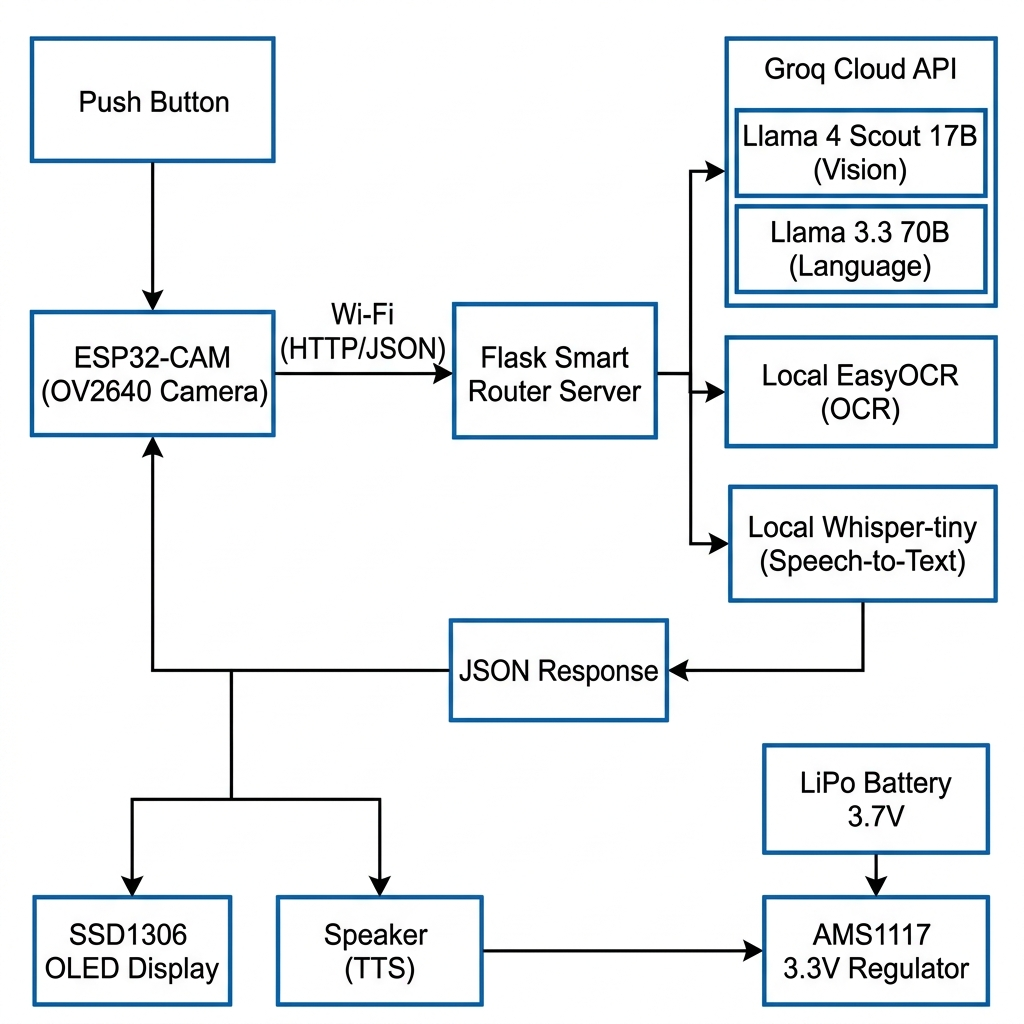
\includegraphics[width=0.85\textwidth]{images/block_diagram.png}
\caption{System Architecture Block Diagram --- AI-Powered Smart Glasses Using ESP32-CAM}
\end{figure}

The block diagram illustrates the complete data flow from user input through AI processing to output delivery. The system is organized into two major domains: the \textit{Wearable Device Domain} (ESP32-CAM with peripherals) and the \textit{Backend Processing Domain} (Flask server with AI models). These domains communicate wirelessly via Wi-Fi using HTTP/REST protocol.

In the Wearable Device Domain, the ESP32-CAM serves as the central hub connecting all hardware peripherals---the OV2640 camera (via 8-bit parallel bus), the INMP441 microphone (via I2S), the SSD1306 OLED display (via I2C), the micro speaker (via DAC/PWM), and the push buttons (via GPIO). The power supply subsystem (LiPo battery, TP4056 charger, AMS1117 regulator) provides regulated 3.3V power to all components.

In the Backend Processing Domain, the Flask Smart Router receives HTTP requests from the ESP32 and dispatches them to the appropriate AI model. Cloud-based models (Llama 4 Scout 17B, Llama 3.3 70B) are accessed via the Groq API over HTTPS, while local models (EasyOCR, Whisper-tiny) run on the backend server's GPU. The Smart Router manages the lifecycle of local models, ensuring memory-efficient operation.

\section{Power Supply Subsystem}
The power supply subsystem will provide stable, regulated power to all electronic components of the smart glasses. It consists of three key components:

\begin{itemize}[leftmargin=1.5cm]
\item \textbf{LiPo Battery (3.7V, 1000 mAh):} The primary energy storage element. Lithium polymer chemistry provides high energy density in a compact, lightweight form factor suitable for wearable applications. The battery will provide a nominal voltage of 3.7V, ranging from 4.2V (fully charged) to 3.0V (minimum safe discharge level).

\item \textbf{TP4056 Charging Module:} Will provide safe, controlled charging of the LiPo battery via USB micro connector. The module implements constant-current/constant-voltage (CC/CV) charging with automatic cutoff at 4.2V to prevent overcharging. Built-in undervoltage protection will disconnect the load at 2.5V to prevent deep discharge damage. A dual-LED indicator (red for charging, blue/green for fully charged) will provide charging status feedback.

\item \textbf{AMS1117-3.3V Voltage Regulator:} Will convert the variable battery voltage (3.0V--4.2V) to a stable 3.3V output required by the ESP32 and all peripheral components. The AMS1117 is a low-dropout (LDO) regulator with 1.1V dropout voltage and 800 mA maximum output current, providing adequate headroom for the system's peak current draw of approximately 346 mA. Two 100nF ceramic decoupling capacitors will be placed near the regulator output and the ESP32 power input pins to suppress high-frequency noise and prevent brownout resets during Wi-Fi transmission bursts, which can cause momentary current spikes of up to 500 mA.
\end{itemize}

\section{ESP32 Control Unit}
The ESP32-CAM module will serve as the central control unit, executing the firmware that orchestrates all hardware interactions and network communications. The dual-core Xtensa LX6 processor will allocate tasks across its two cores for optimal performance:

\begin{itemize}[leftmargin=1.5cm]
\item \textbf{Core 0:} Will handle the Wi-Fi protocol stack, TCP/IP networking, and HTTP client operations. This dedicated allocation ensures that network operations do not interrupt time-sensitive peripheral communication.

\item \textbf{Core 1:} Will run the main application loop, including camera frame capture, I2C display rendering, I2S microphone sampling, GPIO button interrupt handling, JSON parsing, and application state management.
\end{itemize}

The firmware will manage the following operations:

\begin{itemize}[leftmargin=1.5cm]
\item Camera frame buffer allocation and JPEG compression using the ESP32's hardware JPEG encoder
\item I2C bus initialization for the OLED display (SDA: GPIO 14, SCL: GPIO 15) at 400 kHz
\item I2S peripheral configuration for the INMP441 microphone (WS: GPIO 25, SCK: GPIO 26, SD: GPIO 22) at 16 kHz sample rate
\item GPIO interrupt handlers for push button presses (Button 1: GPIO 12, Button 2: GPIO 13) with 200 ms software debouncing
\item HTTP POST client operations for server communication using the ESP32 HTTPClient library
\item JSON response parsing using the ArduinoJson library (v6.x) for extracting AI response text
\item OLED display rendering with automatic word wrapping, scrolling, and mode status indicators
\end{itemize}

\section{Sensor Subsystem}
The system will employ two primary sensing modalities to capture visual and auditory input from the user's environment:

\begin{itemize}[leftmargin=1.5cm]
\item \textbf{Visual Sensor (OV2640 Camera):} Will capture images in JPEG format at 640$\times$480 resolution using the ESP32-CAM's integrated camera module. The camera interfaces with the ESP32 through an 8-bit parallel data bus with four timing signals: XCLK (20 MHz external clock generated by the ESP32), PCLK (pixel clock output from the camera), VSYNC (vertical sync indicating frame boundaries), and HREF (horizontal reference indicating valid pixel data). The camera's built-in auto-exposure (AEC), auto-gain (AGC), and auto-white-balance (AWB) algorithms will ensure consistent image quality across varying lighting conditions---from bright outdoor sunlight to dim indoor environments. The JPEG compression hardware within the OV2640 will reduce raw image data from approximately 600 KB (640$\times$480$\times$2 bytes in RGB565) to approximately 30--50 KB, enabling efficient wireless transmission.

\item \textbf{Audio Sensor (INMP441 Microphone):} Will capture audio data through the I2S digital interface at 16 kHz sample rate with 24-bit resolution per sample. The I2S bus uses three signal lines: WS (Word Select/LRCLK on GPIO 25) to indicate left/right channel selection, SCK (Serial Clock/BCLK on GPIO 26) for bit-level synchronization, and SD (Serial Data on GPIO 22) for the actual audio data stream. The digital MEMS microphone provides 61 dB signal-to-noise ratio, ensuring clear voice capture even in moderately noisy environments. The omnidirectional pickup pattern will capture the user's voice from any direction, accommodating natural speaking positions.
\end{itemize}

\section{OLED Display Subsystem}
The SSD1306 OLED display will be driven via the I2C protocol at device address 0x3C with 400 kHz clock speed, using the Adafruit SSD1306 library for graphics rendering. The display will support three rendering modes:

\begin{itemize}[leftmargin=1.5cm]
\item \textbf{Text Mode:} Will render AI response text using a 6$\times$8 pixel monospace font, providing approximately 21 characters per line and 8 lines per screen. Automatic word wrapping at word boundaries will ensure readable text presentation. Responses exceeding the 8-line capacity will be displayed with automatic vertical scrolling at a configurable speed.

\item \textbf{Status Mode:} Will display the current operating mode (Scene, OCR, Voice, Q\&A, Translate) as a header bar with the battery voltage indicator on the right side. This mode will be active between AI requests, providing the user with feedback about the current system state.

\item \textbf{Processing Mode:} Will display an animated loading indicator while the system is waiting for the AI response from the backend server. This will provide visual feedback that the system is actively processing the request and prevent the user from triggering duplicate requests.
\end{itemize}

The self-emitting OLED technology provides high contrast (10,000:1 ratio) and wide viewing angles (up to 160 degrees), ensuring visibility in both bright outdoor and dim indoor environments. The display draws only 20 mA at full brightness, contributing minimally to overall power consumption.

\section{Flask Web Server (Smart Router)}
The Flask web server will serve as the intelligence hub of the system. It will expose six API endpoints (five functional endpoints plus one health check) and implement the Smart Routing logic that is the core architectural innovation of this project.

\subsection*{Server Architecture Layers:}
The backend server will be organized into four distinct architectural layers, each with clearly defined responsibilities:

\begin{enumerate}[leftmargin=1.5cm]
\item \textbf{Request Handler Layer:} Will receive incoming HTTP POST requests, validate the Content-Type header (application/json), parse the JSON payload, validate the presence of required fields (image data, request type), and extract the Base64-encoded payload for processing. Malformed requests will receive HTTP 400 (Bad Request) responses with descriptive error messages. Requests to undefined endpoints will receive HTTP 404 (Not Found) responses.

\item \textbf{Smart Router Layer:} Will determine the appropriate AI model based on the endpoint called, manage the model loading and unloading lifecycle, and track system resource usage via the psutil library and PyTorch's CUDA memory tracking utilities (\texttt{torch.cuda.memory\_allocated()}, \texttt{torch.cuda.memory\_reserved()}). The router will maintain an internal model registry that tracks which local model (if any) is currently loaded in GPU memory. Before loading a new local model, the router will ensure any previously loaded model is fully unloaded and its memory is freed.

\item \textbf{AI Model Layer:} Will contain wrapper functions for each AI model, providing a unified interface for the Smart Router:
\begin{itemize}
\item Groq API client wrapper for cloud models (Llama 4 Scout 17B for vision, Llama 3.3 70B for language tasks)
\item EasyOCR reader instance wrapper for optical character recognition (supports English and Hindi)
\item Whisper model instance wrapper for speech-to-text transcription
\end{itemize}
Each wrapper function will accept raw input data (decoded image bytes or audio samples) and return a standardized response dictionary containing the AI-generated text and processing metadata.

\item \textbf{Response Layer:} Will format AI model outputs into standardized JSON responses containing four fields: \texttt{status} (success/error string), \texttt{response} (AI-generated text), \texttt{processing\_time\_ms} (elapsed time in milliseconds), and \texttt{memory\_usage\_mb} (current GPU memory allocation in megabytes). This standardized format will enable the ESP32 firmware to parse responses from any endpoint using a single JSON parsing routine.
\end{enumerate}

% =====================================================================
% CHAPTER 7: EXPECTED OUTCOME
% =====================================================================
\chapter{Expected Outcome}

Upon successful completion of the project, the following functional outcomes and performance targets are expected to be achieved:

\section{Functional Outcomes}
\begin{itemize}[leftmargin=1.5cm]
\item A working smart glasses prototype that will capture images through the ESP32-CAM OV2640 camera module and wirelessly transmit them to the Flask backend server for AI processing. The processed AI response will be displayed on the SSD1306 OLED screen (128$\times$64 pixels) with automatic word wrapping and scrolling, and spoken through the micro speaker via text-to-speech conversion.

\item A Flask backend with Smart Routing that will correctly distribute requests between cloud AI models (Groq API --- Llama 4 Scout 17B for vision, Llama 3.3 70B for language processing) and local models (EasyOCR for OCR, Whisper-tiny for speech recognition). The Smart Router will manage model lifecycle automatically, loading models on demand and unloading them after use to optimize memory consumption.

\item Five fully functional AI capabilities accessible through the glasses via the two-button interface:
\begin{enumerate}
\item \textbf{Scene Description} --- The camera will capture an image and the Llama 4 Scout 17B vision model will generate a detailed natural language description of the scene, including objects, people, actions, and spatial relationships.
\item \textbf{Text Extraction (OCR)} --- The EasyOCR model will read and extract printed text from signs, books, documents, labels, and other text-bearing surfaces captured by the camera.
\item \textbf{Speech-to-Text} --- The INMP441 microphone will capture the user's speech and the Whisper-tiny model will transcribe it to text with support for English and other major languages.
\item \textbf{Question Answering} --- The user will be able to ask factual, contextual, or general knowledge questions, and the Llama 3.3 70B language model will generate accurate, informative answers.
\item \textbf{Language Translation} --- Text input (from OCR or speech) will be translated between supported languages (English, Hindi, Kannada, and other languages supported by Llama 3.3 70B).
\end{enumerate}

\item A portable, battery-powered wearable device mounted on a standard glasses frame that will be comfortable for extended wear and operable through simple button presses, requiring no technical expertise from the end user.

\item A dual-output system that will deliver AI responses through both visual (OLED display) and auditory (speaker with TTS) channels simultaneously, accommodating users with varying degrees of visual impairment and different environmental conditions.
\end{itemize}

\section{Expected Performance Metrics}
The following performance metrics are anticipated based on the architectural design, component specifications, and the known performance characteristics of the Groq API infrastructure:

\begin{table}[h]
\centering
\begin{tabular}{|l|c|c|c|}
\hline
\textbf{AI Task} & \textbf{Expected Response} & \textbf{Processing} & \textbf{Memory} \\
 & \textbf{Time} & \textbf{Location} & \textbf{Usage} \\
\hline
Vision (Scene Description) & $<$ 1 second & Groq Cloud API & 0 MB local \\
\hline
Question Answering & $<$ 1 second & Groq Cloud API & 0 MB local \\
\hline
Language Translation & $<$ 1 second & Groq Cloud API & 0 MB local \\
\hline
OCR (Text Extraction) & $<$ 2 seconds & Local (EasyOCR) & $\approx$180 MB \\
\hline
Speech-to-Text & $<$ 1 second & Local (Whisper-tiny) & $\approx$145 MB \\
\hline
\end{tabular}
\caption{Expected Response Time and Resource Usage Metrics}
\end{table}

\section{System-Level Performance Expectations}
\begin{itemize}[leftmargin=1.5cm]
\item \textbf{Peak GPU Memory Usage:} Expected to remain under 600 MB through the Smart Routing architecture, which will ensure that only one local AI model is resident in GPU memory at any given time. This is well within the 4 GB capacity of entry-level NVIDIA GPUs (GTX 1650) and the 8 GB capacity of the RTX 3050.

\item \textbf{API Availability:} The Groq free-tier API provides 14,400 requests per day, which is sufficient for approximately 10 requests per minute sustained over 24 hours. For typical usage patterns (intermittent queries during waking hours), this allowance will support continuous daily use without throttling.

\item \textbf{Network Latency:} On a local Wi-Fi network, HTTP request/response round-trip latency between the ESP32-CAM and the Flask server is expected to be under 50 ms, contributing minimally to the overall response time.

\item \textbf{Battery Life:} The 1000 mAh LiPo battery is expected to provide 2.5--3 hours of continuous active use and 4--5 hours of intermittent use (with idle periods between commands).

\item \textbf{Testing Coverage:} The system is expected to pass all tests across three tiers: AI model accuracy tests (5/5 models), memory management tests (3/3 scenarios), and Flask endpoint integration tests (5/5 endpoints), achieving a 100\% pass rate across all test categories.
\end{itemize}

% =====================================================================
% CHAPTER 8: ADVANTAGES AND FUTURE SCOPE
% =====================================================================
\chapter{Advantages and Future Scope}

\section{Advantages}
The proposed AI-powered smart glasses system will offer the following significant advantages over existing commercial and academic solutions:

\begin{enumerate}[leftmargin=1.5cm]
\item \textbf{Affordable Hardware:} The hardware prototype will use low-cost, readily available electronic components sourced from standard suppliers and online marketplaces. This will make the system significantly more affordable than commercial alternatives such as Google Glass Enterprise Edition and Meta Ray-Ban Smart Glasses, which are priced at levels that exclude most potential users in developing countries. The use of the ESP32-CAM as the central controller, combined with commodity sensors and displays, will ensure that the prototype can be replicated by students, researchers, and humanitarian organizations with limited budgets.

\item \textbf{Zero Operational Cost:} By utilizing the Groq free-tier API (providing 14,400 daily requests at no charge) and open-source local models (EasyOCR under Apache 2.0 license, Whisper under MIT license), the system will incur no recurring subscription fees, cloud computing charges, or software licensing costs. This zero-cost operational model will make the system sustainable for long-term deployment in resource-constrained settings such as schools for the visually impaired, community health centers, and rural rehabilitation programs.

\item \textbf{Memory Efficient Architecture:} The Smart Routing architecture will keep peak GPU memory usage under 600 MB by ensuring that only one local AI model is loaded into GPU memory at any given time. Models will be explicitly unloaded after each request through Python garbage collection and PyTorch CUDA cache clearing. This memory efficiency will enable deployment on entry-level consumer hardware such as laptops with NVIDIA GTX 1650 (4 GB VRAM) or RTX 3050 (8 GB VRAM) GPUs, eliminating the need for expensive server-grade hardware.

\item \textbf{Multi-Modal AI Capabilities:} The system will integrate five distinct AI modalities---computer vision (scene description), natural language processing (question answering and translation), optical character recognition (text extraction), and automatic speech recognition (voice-to-text)---within a single wearable device. This comprehensive multi-modal capability will provide users with a versatile assistive tool that addresses a wide range of daily challenges faced by visually impaired individuals.

\item \textbf{Fast Response Times:} All AI tasks will be designed to complete within 2 seconds, providing near-real-time assistance to the user. Cloud-based tasks (scene description, Q\&A, translation) leveraging Groq's high-performance inference infrastructure are expected to complete in under 1 second. This responsiveness will ensure that the system feels natural and intuitive to use, encouraging sustained adoption.

\item \textbf{Scalable Architecture:} The Flask backend will be capable of serving multiple smart glasses clients simultaneously, as each request is handled independently and stateless. The cloud-local workload distribution can be dynamically adjusted based on network availability---falling back to local-only processing when internet connectivity is unavailable, or shifting more tasks to the cloud when bandwidth permits.

\item \textbf{Open-Source Software Stack:} The entire software stack will use open-source technologies (Python, Flask, EasyOCR, Whisper, PyTorch), eliminating vendor lock-in and enabling community contributions. The source code, firmware, and design documentation will be made available for replication and extension by the academic and open-source communities.

\item \textbf{Dual Output Modalities:} AI responses will be delivered through both visual (OLED display with text rendering) and auditory (micro speaker with text-to-speech) channels simultaneously. This dual-output approach will accommodate users with varying degrees of visual impairment---from partially sighted users who can read the OLED display to completely blind users who will rely exclusively on the audio output. It will also adapt to different environmental conditions (e.g., noisy environments where audio is impractical, or quiet settings where screen reading is preferred).
\end{enumerate}

\section{Future Scope}
The modular architecture of the proposed system will enable several enhancements and extensions in future iterations:

\begin{enumerate}[leftmargin=1.5cm]
\item \textbf{Real-Time Object Detection:} Integration of lightweight object detection models such as YOLOv8-nano or MobileNet-SSD for continuous real-time object identification and obstacle warning. This will enable the glasses to proactively alert the user about objects, people, and potential hazards in their path without requiring manual trigger via button press.

\item \textbf{GPS Navigation Assistance:} Adding a GPS module (such as NEO-6M or BN-880) and integrating with mapping APIs (Google Maps, OpenStreetMap) will enable turn-by-turn navigation assistance for visually impaired users. Audio-guided walking directions combined with landmark identification via the camera will provide comprehensive outdoor navigation support.

\item \textbf{Multi-Language Voice Commands:} Extending the Whisper integration to support voice commands in regional Indian languages including Kannada, Hindi, Tamil, Telugu, and Malayalam. This will make the system accessible to users who are not proficient in English, significantly expanding the potential user base in India's linguistically diverse population.

\item \textbf{Custom PCB Design:} Replacing the breadboard/jumper wire prototype with a custom-designed printed circuit board (PCB) will significantly reduce the device's physical size, weight, and power consumption while improving electrical reliability. A two-layer or four-layer PCB with surface-mount components will enable a more professional and durable form factor suitable for daily use.

\item \textbf{Mobile App Companion:} Developing a companion Android/iOS application that will provide remote configuration of the smart glasses settings, usage analytics and history, real-time monitoring, and caregiver alerts. The mobile app will communicate with the glasses via Bluetooth Low Energy (BLE), enabling features such as remote firmware updates and GPS sharing.

\item \textbf{Battery Optimization and Sleep Modes:} Implementing deep sleep modes on the ESP32 and wake-on-button interrupt will dramatically reduce idle power consumption from approximately 160 mA to under 10 $\mu$A. This optimization is expected to extend battery life from 3 hours of continuous use to 8--10 hours of intermittent use, making the device practical for all-day wear.

\item \textbf{Edge AI Processing:} Porting lightweight AI models (such as TensorFlow Lite Micro models for basic object classification) to run directly on the ESP32-S3 (which includes vector instruction extensions and PSRAM support) will enable basic offline AI functionality without requiring any server connectivity. This will make the system functional in areas with no Wi-Fi coverage, such as outdoor environments and rural areas.
\end{enumerate}

% =====================================================================
% CHAPTER 9: CONCLUSION AND REFERENCES
% =====================================================================
\chapter{Conclusion}

This project proposes the design and implementation of AI-powered smart glasses that will deliver advanced capabilities including image understanding, text extraction, speech recognition, question answering, and language translation through an affordable wearable device built using readily available electronic components. The system will be built around the ESP32-CAM microcontroller, which provides an integrated camera, Wi-Fi connectivity, and sufficient processing power for real-time image capture and wireless data transmission in a compact, low-power form factor.

The hybrid cloud-local AI architecture to be implemented through the Flask Smart Router represents the key technical contribution of this project. By offloading computationally intensive vision and language tasks to the Groq free-tier cloud API---utilizing Llama 4 Scout 17B for multimodal image description and Llama 3.3 70B Versatile for question answering, translation, and text generation---while processing lightweight OCR and speech recognition tasks locally using EasyOCR and OpenAI Whisper-tiny respectively, the system will achieve a practical balance between performance, operational cost (zero recurring charges), and resource utilization that has not been demonstrated in prior academic work.

The Smart Routing memory management strategy will ensure that only one local AI model occupies GPU memory at any given time, with explicit model unloading after each request through Python garbage collection and PyTorch CUDA cache clearing. This approach is designed to maintain peak RAM usage at approximately 600 MB, making the system compatible with entry-level NVIDIA GPUs such as the GTX 1650 (4 GB) and RTX 3050 (8 GB). Without this optimization, loading all four AI models simultaneously would require over 12 GB of VRAM, rendering the system impractical for deployment on any consumer-grade hardware.

The system will be designed to achieve response times under 2 seconds for all five AI tasks, with cloud-based tasks expected to complete in under 1 second (leveraging Groq's optimized inference infrastructure) and local tasks expected to complete in under 2 seconds. The dual-output design---combining an SSD1306 OLED display for visual text rendering and a micro speaker for text-to-speech audio feedback---will ensure accessibility for users with varying degrees of visual impairment. Comprehensive testing will be conducted across three tiers: AI model accuracy tests, memory management tests, and Flask endpoint integration tests, aiming for a 100\% pass rate across all categories.

The project aims to demonstrate that the combination of affordable IoT hardware, free-tier cloud AI services, and intelligent software architecture can democratize access to AI-powered assistive technology. By using readily available, low-cost components and freely accessible cloud AI models, the system will prove that advanced assistive technology need not be expensive or require specialized hardware, potentially making it accessible to visually impaired users in developing countries and underserved communities who currently have no access to such technology. The modular and extensible architecture will ensure that the system can be enhanced with additional AI capabilities, hardware sensors, navigation features, and output modalities as technology continues to evolve and new models become available.

% =====================================================================
% REFERENCES
% =====================================================================
\chapter{References}

\begin{enumerate}[leftmargin=1.5cm]
\item S. Das, S. Saxena, and N. K. Rout, ``Low Cost Smart-Glass using ESP-32,'' in \textit{2021 IEEE 2nd International Conference on Applied Electromagnetics, Signal Processing, \& Communication (AESPC)}, Bhubaneswar, India, 2021, pp. 1--5.

\item S. S. V. Ramesh Babu, M. Gowtham, G. Jayakrishna, and A. L. S. S. Manasa, ``AI-Powered Smart Glasses For The Blind Using OpenCV \& Python,'' in \textit{2025 IEEE Wireless Antenna and Microwave Symposium (WAMS)}, Visakhapatnam, India, 2025, pp. 1--4.

\item J. Y. Lin, C. C. Yao, C. L. Chiang, and M. C. Chen, ``Smart Glasses Application System for Visually Impaired People Based on Deep Learning,'' in \textit{Indo-Taiwan 2nd International Conference on Computing, Analytics and Networks (Indo-Taiwan ICAN)}, Rajpura, India, 2020, pp. 178--182.

\item A. Radford, J. W. Kim, T. Xu, G. Brockman, C. McLeavey, and I. Sutskever, ``Robust Speech Recognition via Large-Scale Weak Supervision,'' in \textit{Proceedings of the 40th International Conference on Machine Learning (ICML)}, Honolulu, HI, USA, vol. 202, 2023, pp. 28492--28518.

\item H. Touvron, L. Martin, K. Stone, et al., ``Llama 2: Open Foundation and Fine-Tuned Chat Models,'' \textit{Meta AI Research}, arXiv:2307.09288, 2023.

\item JaidedAI, ``EasyOCR: Ready-to-Use OCR with 80+ Supported Languages and All Popular Writing Scripts,'' \textit{GitHub Repository}, 2020. [Online]. Available: \url{https://github.com/JaidedAI/EasyOCR}

\item N. Gospodinov and G. Krastev, ``Object detection with smart glasses,'' in \textit{2022 30th National Conference with International Participation (TELECOM)}, Sofia, Bulgaria, Oct. 2022, pp. 49--52.

\item P. Sharma, M. Sadasivan, A. S. Babu, and K. T. A. Robert, ``Smart Glasses for the Blind: A Real-Time AI-Driven Wearable System for Autonomous Navigation,'' in \textit{2025 International Conference on Computing and Communications (COMPUTINGCON)}, Pune, India, Sep. 2025, pp. 1--6.

\item U. R, H. P.S., R. N.G., and N. A, ``Third Eye -- A Smart Wearable Glass With Deep Learning Technology Powered With Artificial Intelligence for Visually Impaired People,'' in \textit{2023 IEEE International Students' Conference on Electrical, Electronics and Computer Science (SCEECS)}, Bhopal, India, Feb. 2023, pp. 1--5.

\item J. Chen and X. Ran, ``Deep Learning with Edge Computing: A Review,'' in \textit{Proceedings of the IEEE}, vol. 107, no. 8, pp. 1655--1674, Aug. 2019.

\item Espressif Systems, ``ESP32-CAM Module Technical Reference Manual,'' Version 4.0, 2020. [Online]. Available: \url{https://www.espressif.com/sites/default/files/documentation/esp32_technical_reference_manual_en.pdf}

\item Groq Inc., ``GroqCloud API Reference Documentation,'' Version 1.0, 2024. [Online]. Available: \url{https://console.groq.com/docs/api-reference}
\end{enumerate}


\end{document}
